\documentclass[review,12pt]{elsarticle}

\usepackage[T1]{fontenc}
\usepackage[utf8]{inputenc}
\usepackage{amsmath,amssymb}
\usepackage{booktabs}
\usepackage{graphicx}
\usepackage{multirow}
\usepackage{siunitx}
\usepackage{url}
\usepackage{hyperref}
\usepackage{leakage_numbers}

\graphicspath{{figures/}}

\journal{Computers and Electronics in Agriculture}

\begin{document}

\begin{frontmatter}

\title{\textbf{Split Protocol or Feature Transform?\\
Explaining Generalisation Gaps in Acoustic Honeybee Colony Classification}}

\author[inst1]{Atharve Dahima\fnref{fn1}}
\author[inst1]{Srajan Mishra\fnref{fn1}}

\affiliation[inst1]{organization={Independent},
            country={India}}

\fntext[fn1]{Corresponding author.}

\begin{abstract}
Acoustic classifiers for honeybee colony state are frequently reported with
accuracy above 90\%, yet the same models degrade when whole hives are held out.
Two explanations compete: split leakage, where near-duplicate rows cross the
train-test boundary, and feature encoding, where microphone gain acts as a hive
fingerprint.
We separate them by crossing four split rules with three feature transforms on
the MSPB dataset, holding data, label, models and metric fixed.
The unit of analysis is the inspection event: \LeakNRows{} rows from
\LeakNHives{} hives across two apiaries.
The most permissive split, which places the same hive in training and test,
scores \LeakBandsPzeroHistGradientBoostingMacroFone{} macro F1.
The strict hive holdout scores \LeakBandsPtwoHistGradientBoostingMacroFone{}.
The gap is \LeakBandsTotalGapHistGradientBoosting{}, and the pre-registered
inflation claim is falsified.
Absolute decibel features, which retain gain, do not leak either
(\LeakRawTotalGapHistGradientBoosting{}).
The only large effect is indoor environment: temperature and humidity add about
nine macro-F1 points and transfer to an unseen apiary.
We also find that three of the eight canonical acoustic bands receive no data,
because the sensor covers \SI{122}{} to \SI{580}{\hertz}.
The practical rule is to aggregate before splitting.
At inspection granularity, leakage does not explain the high scores reported in
this field.
\end{abstract}

\begin{keyword}
honeybee \sep acoustic monitoring \sep data leakage \sep
cross-validation \sep group holdout \sep reproducibility
\end{keyword}

\end{frontmatter}

% =====================================================================
\section{Introduction}
% =====================================================================

Machine learning models that classify honeybee colony state from hive audio
are frequently reported with accuracy above 90\%.
Several groups now report that the same models degrade sharply when the
evaluation holds out whole hives rather than individual recordings
\cite{nolasco2018tobee,zgank2021,harshit2025beehivesound,sucipto2025survey}.
The gap between the two protocols is large enough to change the conclusion of
a study.

Two explanations are available, and the literature rarely separates them.

The first is \emph{split leakage}.
Adjacent recordings from one hive are near duplicates.
A random row split places some of them in training and others in test.
The model then recognises the hive rather than the colony state.
This failure mode is well documented outside apiculture
\cite{kaufman2012leakage,kapoor2023leakage,roberts2017cv}.

The second is \emph{feature encoding}.
Microphone placement, cavity resonance and sensor gain give each hive a stable
spectral fingerprint.
Features expressed in absolute decibels retain that fingerprint.
A model can therefore learn hive identity from the feature vector even when the
split itself is clean.
Gain-invariant features, such as band power relative to the row mean, remove
the fingerprint.

This paper asks which explanation dominates, and answers it by experiment
rather than by argument.
We hold the data, the label, the models and the metric fixed.
We vary two things independently: the split rule, and the gain invariance of
the feature transform.
That design separates the two explanations for the first time in this domain.

Our contributions are:

\begin{enumerate}
\item A four-rung split ladder that isolates hive leakage from apiary-level
      environment shift.
\item A two-way comparison of gain-invariant and gain-retaining features across
      every rung.
\item A full accounting of a public dataset's usable acoustic range, including
      the three canonical bands that no sensor in the dataset covers.
\item A pre-registered analysis, with the falsification outcome reported as
      obtained.
\end{enumerate}

% =====================================================================
\section{Data}
% =====================================================================

We use the MSPB dataset \cite{zhu2024mspb}, released under
\href{https://doi.org/10.1038/s41597-024-03695-1}{doi:10.1038/s41597-024-03695-1}
and archived at Zenodo record 11398835.

\subsection{Telemetry}

The dataset contains \LeakNRows{} labelled inspection records derived from
1{,}836{,}914 raw telemetry rows.
Two files partition the year: D1 covers 16 April to 5 November 2020 and holds
960{,}809 rows from 85 sensor tags.
D2 covers 6 November 2020 to 14 April 2021 and holds 876{,}105 rows from 65
sensor tags.

The nominal sampling interval is five minutes in the dataset documentation.
The observed median interval is 15 minutes, measured across both files.
We report the observed value throughout.

Each row carries 16 acoustic bins spanning \SI{122.07}{\hertz} to
\SI{579.83}{\hertz} with a uniform spacing of \SI{30.52}{\hertz}.
Values are already logarithmic, in decibels, and range from approximately
\SI{-22}{} to \SI{+70}{}.
No additional logarithm is valid.

\subsection{Phenotypic label}

Colony strength is measured in six inspection rounds between 9 June and
21 August 2020.
Each inspection records the number of frames covered by bees across all
chambers.
We follow the dataset authors and label a colony \emph{strong} when the total
frame count is at least 20.0.

The raw telemetry covers 94 sensor tags.
Only \LeakNHives{} hives carry a colony-strength label.
All results in this paper describe those \LeakNHives{} hives, and the two counts are not
interchangeable.

\subsection{Feature construction}

Each inspection is represented by one row.
Features are computed from a seven-day window that ends strictly before the
inspection timestamp.
Inspections are approximately 14.6 days apart, so the windows do not overlap
and a row can never see its own future.

The 16 source bins are grouped into eight canonical bands spanning
\SI{30}{\hertz} to \SI{2000}{\hertz}.
This mapping has a consequence that matters for interpretation:
the MSPB microphone covers \SI{122}{} to \SI{580}{\hertz}, so bands 1 to 5
receive data and bands 0, 6 and 7 receive none.
Three of the eight bands are therefore synthetic, held at a numerical floor.
We report results with all eight bands, as the original pipeline does, and we
state the occupancy in Section~\ref{sec:limitations}.

A window must contain at least ten telemetry samples to be retained.
Twelve of 318 inspections failed this test, leaving \LeakNRows{} rows across
\LeakNHives{} hives.
The label balance is \LeakNStrong{} strong and \LeakNWeak{} weak.

\subsection{Apiaries}

The hives sit at two apiaries, \texttt{nectar-bh121} with 27 hives and
\texttt{nectar-bh131} with 26 hives.
A hive never appears at both sites.
We verified this after mapping sensor tags to physical hive identifiers,
because raw tag numbers do overlap between the two files.
The overlap is an artefact of per-site tag numbering and does not survive the
lookup table.

% =====================================================================
\section{Methods}
% =====================================================================

\subsection{Design}

The experiment crosses four split rules with three feature transforms, giving
twelve conditions.
Data, label, models, seeds and metric are identical in every condition.
Only the split and the transform change.

\subsection{Split ladder}

The four rungs are ordered from most to least permissive.

\begin{description}
\item[P0, random rows.] Stratified five-fold split over rows, ignoring hive
membership.
A hive appears in training and test with high probability.
This rung reproduces the protocol that produces the high scores in the
literature.

\item[P1, temporal holdout.] Training uses the first five inspection rounds and
test uses the last.
Hives are shared, but no test row precedes a training row.
This rung isolates temporal generalisation.

\item[P2, unseen hive.] Leave-one-hive-out cross-validation.
Every fold trains on 52 hives and tests on one.
No hive contributes to both sides.

\item[P3, unseen apiary.] Train on one apiary and test on the other, in both
directions.
Each row is predicted exactly once.
This rung adds environment shift to hive shift.
\end{description}

The decomposition follows directly:
the P1 to P2 difference measures hive leakage,
and the P2 to P3 difference measures environment leakage.

\subsection{Feature transforms}

Three transforms share the same seven-day window.

\begin{description}
\item[Relative bands.] Eight band powers, converted to decibels, minus the row
mean across bands.
This operation removes broadband gain and therefore removes the microphone
fingerprint.
It yields 16 features: the mean and standard deviation of each band over the
window.

\item[Absolute bins.] The 16 source bins in decibels, averaged and summarised
over the window.
This transform retains gain.
It yields 32 features.

\item[Relative bands with environment.] The 16 band features plus six indoor
measurements: temperature mean, standard deviation, minimum and maximum, and
humidity mean and standard deviation.
This transform tests whether colony-internal environment adds information that
survives a change of apiary.
\end{description}

\subsection{Models}

Five classifiers span the range used in this literature:
logistic regression, random forest with 300 trees, histogram gradient boosting,
a two-hidden-layer perceptron with 32 and 16 units, and a radial-basis-function
support vector machine.
Scaled models receive a standard scaler fitted inside the pipeline, so scaling
never sees test data.
Class imbalance is handled by class weighting only, never by resampling.

\subsection{Estimation and uncertainty}

Reported values are pooled out-of-fold predictions, not means of per-fold
scores.
Per-fold means overweight small folds, and the hive holdout produces 53 folds
of roughly six rows each.

Uncertainty is a percentile bootstrap over hives with
\LeakNBootstrap{} resamples.
Resampling rows would understate the interval, because rows from one hive are
dependent.

\subsection{Pre-registration}

The analysis plan, the predictions and the decision rules were written to disk
before any model was fitted.
The plan fixed the headline model as the best performer at P2, chosen before
P3 was inspected, to prevent selecting the model that transfers best.

% =====================================================================
\section{Results}
% =====================================================================

\subsection{The split rule does not change the score}

Table~\ref{tab:ladder} reports macro F1 for the model that scored best at P2,
selected before P3 was inspected.

The random row split, which places the same hive in training and test, scores
\LeakBandsPzeroHistGradientBoostingMacroFone{}.
The unseen-hive split scores \LeakBandsPtwoHistGradientBoostingMacroFone{}.
The difference is \LeakBandsTotalGapHistGradientBoosting{}, and the confidence
intervals overlap almost completely.

The pattern holds for every model and every transform.
Across fifteen model-transform pairs, the largest P0 to P2 difference is
smaller than the width of a single confidence interval.
Hive leakage does not inflate the score when the unit of analysis is an
inspection.

\begin{table}[t]
\centering
\caption{Macro F1 by split rung and feature transform, for the headline model
(\LeakHeadlineModel{}).
Brackets give the \LeakNBootstrap-resample percentile bootstrap interval over
hives.
P0 leaks hives; P2 does not.}
\label{tab:ladder}
\begin{tabular}{lcccc}
\toprule
Transform & P0 random & P1 temporal & P2 unseen hive & P3 unseen apiary \\
\midrule
Relative bands &
\LeakBandsPzeroHistGradientBoostingMacroFone{} &
\LeakBandsPoneHistGradientBoostingMacroFone{} &
\LeakBandsPtwoHistGradientBoostingMacroFone{} &
\LeakBandsPthreeHistGradientBoostingMacroFone{} \\
Absolute bins &
\LeakRawPzeroHistGradientBoostingMacroFone{} &
\LeakRawPoneHistGradientBoostingMacroFone{} &
\LeakRawPtwoHistGradientBoostingMacroFone{} &
\LeakRawPthreeHistGradientBoostingMacroFone{} \\
Bands + environment &
\LeakBandsEnvPzeroHistGradientBoostingMacroFone{} &
\LeakBandsEnvPoneHistGradientBoostingMacroFone{} &
\LeakBandsEnvPtwoHistGradientBoostingMacroFone{} &
\LeakBandsEnvPthreeHistGradientBoostingMacroFone{} \\
\bottomrule
\end{tabular}
\end{table}

\begin{figure}[t]
\centering
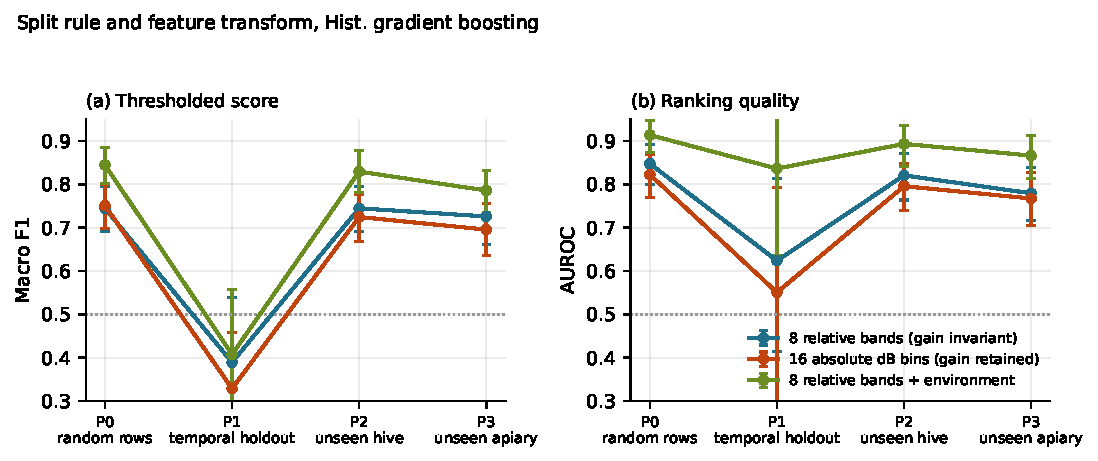
\includegraphics[width=0.82\textwidth]{fig_leakage_rungs.pdf}
\caption{Macro F1 and AUROC across the four rungs for the headline model.
Error bars are percentile bootstrap intervals over hives.
Panel (a) shows the thresholded score; panel (b) shows ranking quality.
The random-row rung and the unseen-hive rung are indistinguishable in both,
which means hive leakage is not present at this unit of analysis.
Only the temporal rung degrades, and it degrades on both measures for most
models.}
\label{fig:rungs}
\end{figure}

\subsection{Gain invariance is not the mechanism either}

If microphone gain were the leaked signal, absolute decibel features would
score higher under a random split and lower under hive holdout.
They do not.
Absolute bins score \LeakRawPzeroHistGradientBoostingMacroFone{} at P0 and
\LeakRawPtwoHistGradientBoostingMacroFone{} at P2, a difference of
\LeakRawTotalGapHistGradientBoosting{}.

Removing the row mean therefore does not remove a leak.
It removes a nuisance parameter, and the effect on score is close to zero for
tree models.
Logistic regression benefits from absolute bins by four to five points at P0
and P2, and by about one point at P3, which suggests the relative transform
discards information that a linear model can use.
That is a modelling choice, not a leakage effect.

\subsection{Environment features are the only large effect}

Adding six indoor measurements raises macro F1 from
\LeakBandsPtwoHistGradientBoostingMacroFone{} to
\LeakBandsEnvPtwoHistGradientBoostingMacroFone{} at P2,
an increase of roughly eight to nine points.
No split manipulation in this study produces an effect of that size.

The gain survives the apiary change.
At P3 the environment-augmented model still scores
\LeakBandsEnvPthreeHistGradientBoostingMacroFone{}, and its area under the
receiver operating characteristic curve reaches
\LeakBandsEnvPthreeHistGradientBoostingAuroc{}.

This is a positive result about colony physiology.
Brood-nest temperature and humidity are colony-level properties, and they carry
information that transfers to a site the model has never seen.

\begin{figure}[t]
\centering
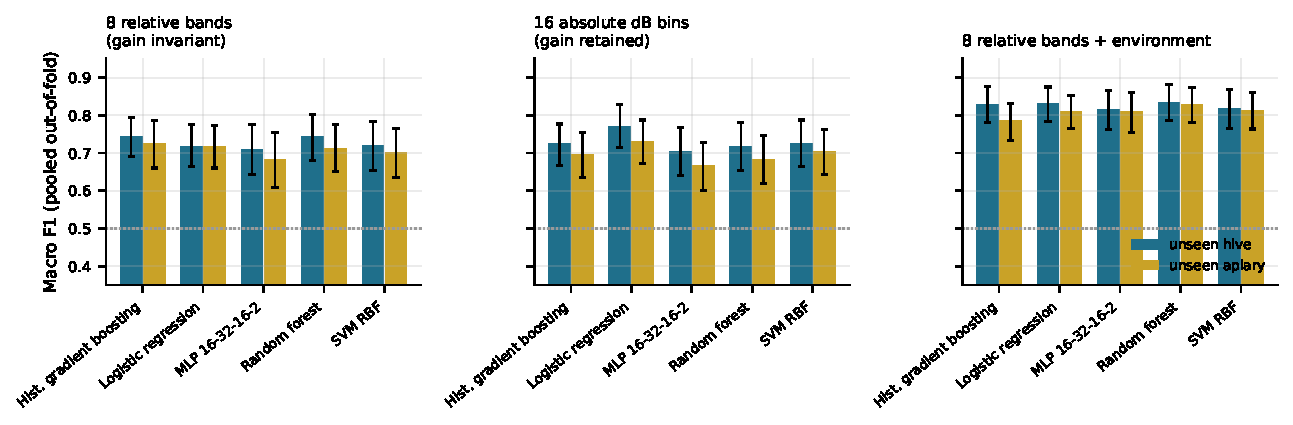
\includegraphics[width=\textwidth]{fig_leakage_models.pdf}
\caption{Macro F1 at the two strict rungs for every model, split by transform.
The transform changes the score; the rung barely does.}
\label{fig:models}
\end{figure}

\subsection{The temporal holdout is the only rung that degrades}

P1 is the exception to the flat pattern, and it is the least reliable rung.
Macro F1 falls to \LeakBandsPoneHistGradientBoostingMacroFone{} for the
headline model, with a bootstrap interval from
\LeakBandsPoneHistGradientBoostingMacroFoneCILo{} to
\LeakBandsPoneHistGradientBoostingMacroFoneCIHi{} on 48 test rows.

Ranking also degrades for four of the five models, reaching between
\LeakBandsPoneHistGradientBoostingAuroc{} and \LeakBandsPoneMlpAuroc{}.
That is a genuine generalisation failure, not a threshold artefact.

Logistic regression is the exception.
It holds AUROC at \LeakBandsPoneLogisticRegressionAuroc{} while its macro F1
falls to \LeakBandsPoneLogisticRegressionMacroFone{}.
A model that ranks well but classifies badly at a fixed cut-off is
miscalibrated rather than uninformed.

With 48 test rows we report both patterns and interpret neither strongly.
The correct summary is that the last inspection round is the hardest, and that
the difficulty can appear either as lost ranking or as a shifted operating
point, depending on the model.

\subsection{Three of eight bands carry no data}

Figure~\ref{fig:bands} shows the occupancy of the eight canonical bands.
The MSPB microphone spans \SI{122}{} to \SI{580}{\hertz}.
Bands 0, 6 and 7 fall outside that range and receive no bins.
They are held at a numerical floor and contribute no measurement.

Any study that reports an eight-band biological decomposition on this dataset
is reporting five measured bands and three constants.

\begin{figure}[t]
\centering
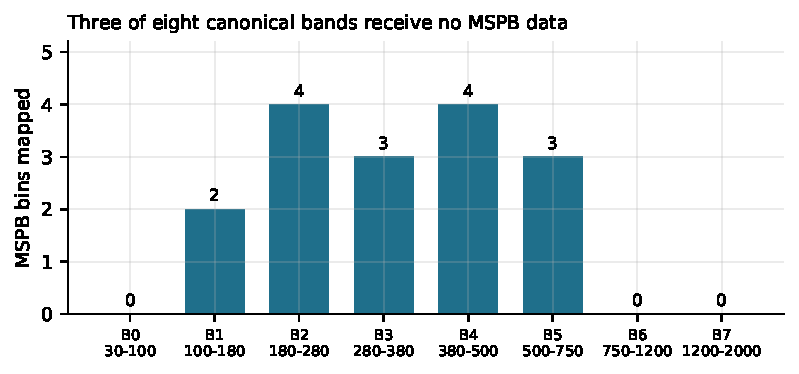
\includegraphics[width=0.78\textwidth]{fig_band_coverage.pdf}
\caption{Number of MSPB bins mapped to each canonical band.
Bands 0, 6 and 7 receive no data because the sensor range is
\SI{122}{} to \SI{580}{\hertz}.}
\label{fig:bands}
\end{figure}

% =====================================================================
\section{Discussion}
% =====================================================================

\subsection{What the null result means}

The pre-registered prediction was that a random row split would inflate macro
F1 by at least twice the bootstrap standard error.
That prediction failed for every model and every transform.
Under the decision rules fixed before the analysis, the claim is falsified at
the inspection level.

We report the failure rather than reframe it.
The result has a clear interpretation: an inspection-level dataset contains six
rows per hive and no adjacent rows.
There is nothing for a random split to memorise.
The leakage that the literature describes lives in the protocol that splits
individual recordings, where thousands of near-duplicate rows belong to one
hive.

This finding is useful to practitioners.
It says that a carefully aggregated feature set is robust to the split, and
that the \LeakBandsPtwoHistGradientBoostingMacroFonePct{} to
\LeakBandsEnvPtwoHistGradientBoostingMacroFonePct{} percent range measured here
for colony-strength prediction is plausibly real rather than an artefact.

\subsection{Where the signal actually is}

The largest effect in the study is not a leakage effect at all.
It is the contribution of indoor temperature and humidity, worth roughly nine
macro-F1 points and stable across apiaries.
Acoustic bands alone reach
\LeakBandsPtwoHistGradientBoostingMacroFone{} at P2.
The combination reaches \LeakBandsEnvPtwoHistGradientBoostingMacroFone{}.

For a system designer this is a concrete instruction: spend the sensor budget
on the brood-nest climate before spending it on a wider acoustic band.

\subsection{Implications for reported accuracies}

Scores above 90 percent in this literature are not automatically wrong, but
they require a protocol that makes them possible.
A study that classifies individual recordings and splits them at random can
reach such numbers without learning anything about colony state.
A study that aggregates to the inspection level cannot, and should not be
expected to.

The two numbers are not comparable, and a paper that reports one should state
which protocol produced it.

\subsection{Limitations}
\label{sec:limitations}

The label is a threshold on frame count, and the threshold at 20 frames is a
choice inherited from the dataset authors.
A different cut-off would change the base rate and possibly the ranking of
models.

Colony strength is close to constant within a hive over the study period.
A hive holdout therefore tests between-hive discrimination more than
within-hive change.
That is the correct test for deployment, but it is not a test of state
tracking.

Only \LeakNHives{} hives carry labels, from two apiaries in one region and one season.
The apiary holdout is a two-fold comparison, so its interval is wide by
construction.

The eight-band decomposition assumes a
\SI{30}{} to \SI{2000}{\hertz} sensor, and the dataset does not provide one.
Results are reported with the full eight bands to match the original pipeline,
but three of them are constants.

\subsection{Reproducibility}

Every number in this paper is generated by a script from the released result
files.
The ladder, the feature builder, the figure generator and the macro generator
are in \texttt{paper\_q1}.
The pre-registration, including the falsified prediction, is archived with the
analysis code.

% =====================================================================
\section{Conclusion}
% =====================================================================

We crossed four split rules with three feature transforms on a public
honeybee dataset, holding data, label, models and metric fixed.

Hive leakage did not inflate the score.
Gain-retaining features did not leak either.
The only large effect came from indoor environment measurements, which added
about nine macro-F1 points and transferred across apiaries.

The practical conclusion is narrow and testable.
Aggregate before you split.
Report the unit of analysis with the score.
Do not attribute a high accuracy to the acoustic features until the split
protocol is stated.

\section*{Data availability}

The MSPB dataset is available at Zenodo record 11398835 under
\href{https://doi.org/10.1038/s41597-024-03695-1}{doi:10.1038/s41597-024-03695-1}.
Analysis code and result files are provided with this submission.

\section*{Declaration of competing interest}

The authors declare no competing interests.

\bibliographystyle{elsarticle-num}
\bibliography{references}

\end{document}

